\chapter{Methods}
\label{chap:methods}
{\color{red}
\Cref{chap:dataplat} introduced a reference architecture for domain-level data platforms, organized around a small set of composable modules -- ingestion, storage, data processes, management, and exploitation -- and distinguished, within the data processes module, between platform processes, maintained by the platform itself, and user processes, the application-specific pipelines through which individual Digital Twins consume and produce data. That architecture, however, is deliberately abstract: it specifies which functionalities a data platform must provide, not which concrete technology should implement each of them. In practice, cloud providers such as Amazon, Google, and Microsoft expose ecosystems of dozens of overlapping, interoperable services, and selecting the right subset for a given application is, in current practice, left to the expertise of individual designers or consultants -- an unstructured, largely non-reproducible process, at odds with the standardization this thesis has argued for throughout.

This chapter addresses this gap, presenting a methodology that systematizes the selection of the concrete services instantiating the modules of a data platform, driven directly by the data-intensive processes the platform is meant to support. In terms of the platform/user process distinction introduced in \Cref{sec:dataplat-refarch}, the methodology takes as input a description of an application's user processes -- for a Digital Twin, its own analytical or operational data pipelines -- and derives, systematically rather than by expert intuition alone, the subset of services from a given ecosystem that implements them at minimal cost, while respecting dependency, compatibility, and mandatory constraints the designer may impose. Fittingly, the resulting characterization of a data platform is the same one adopted throughout this thesis (\Cref{chap:data_oriented_perspective}): a centralized infrastructure providing independent and composable services meeting the end-to-end needs of data pipelines.
}

\section{Data as a blueprint - Process driven design of Data Platforms}
\label{sec:process-driven-design}



Data platforms are state-of-the-art solutions to implement data-driven applications and analytics, since they facilitate the ingestion, storage, management, and exploitation of big data. Data platforms are built on top of complex ecosystems of services answering different data needs and requirements; such ecosystems are offered by different providers (e.g., Amazon AWS and Microsoft Azure). However, when it comes to engineering data platforms, no unifying strategy and methodology is available yet, and the design is mainly left to the expertise of practitioners in the field. Service providers simply expose a long list of interoperable and alternative engines, making it hard to select the optimal subset without a deep knowledge of the ecosystem. A more effective approach to the design starts from the knowledge of the data transformation and exploitation processes that should be supported by the platform. We sketch a computer-aided design methodology and then focus on the selection of the optimal services needed to implement such processes. We show that our approach lightens the design of data platforms and enables an unbiased selection and comparison of solutions even through different service ecosystems.

\subsection{Introduction}

Digital transformation is one of the most disruptive trends of recent years. Digitization is perceived as the most effective solution to innovate every industrial sector thanks to process automation and the (automatic) exploitation of the value hidden in data. Such evolution is pushing information systems towards complex ecosystems of data-oriented services answering different data needs and requirements.

{\color{red}As already characterized in \Cref{chap:data_oriented_perspective}, }a data platform is a centralized infrastructure that facilitates the ingestion, storage, management, and exploitation of large volumes of heterogeneous data. It provides a collection of independent and composable services meeting the end-to-end needs of data pipelines, where: \textit{centralized} means that a data platform is conceptually a single and unified component; \textit{independent} means that changes in the implementation of a service do not affect other services; \textit{composable} means that services have interfaces that enable an easy and frictionless composition; and \textit{end-to-end} means that services cover the entire data life cycle. Data platforms foster collaboration and shared governance (being centralized, data is unified following some integration and it is easier to ensure compliance with data protection and privacy laws through shared security and access control), and scalability (being implemented on a distributed infrastructure, it is easy to add storage and computing resources as needed).

When it comes to building data platforms, no unifying strategy and methodology is there yet: building data platforms is mainly left to the expertise of practitioners or consultancy companies. On the one hand, cloud service providers\footnote{While data platforms are not mandatorily coupled with cloud computing, cloud computing is proving to be a winning business model since deploying and maintaining such a variety of computational resources and assets requires advanced technical skills that companies hardly have ``in-house''.} offer ecosystems of services composed of many engines interoperable with each other; however, choosing the optimal set of services is hard since multiple solutions could fulfill the desiderata (e.g., whether disjoint databases and data warehouses or a single Lakehouse \cite{DBLP:conf/cidr/Zaharia0XA21} should be used) and could require vertical knowledge on the design of data pipelines. On the other hand, several abstract big data architectures have been introduced (e.g., NIST \cite{chang2019nist}, Lambda \cite{DBLP:conf/bigdataconf/KiranMMDB15}, and Kappa \cite{kreps2014questioning}). However, while they provide the necessary functionalities to enable big-data applications, their implementation and adoption require to understand which services should be used.

Neither providers of service ecosystems nor abstract architectures answer a crucial question: \textit{given an ecosystem of services and the data-driven processes to support, which is the optimal subset of services enabling such processes?} Answering this question is hard since (i) each provider offers many (overlapping) services, (ii) different providers offer different service categorizations that can hardly be mapped together, (iii) the evolution of cloud ecosystems is fast and stakeholders without vertical technical knowledge can hardly keep up with the pace, and (iv) simply selecting ``all'' engines is not viable due to cost and management reasons. We believe that to ease the data platform design, the description of data-driven processes should drive such activity. Indeed, data pipelines are the backbone of a \textit{data} platform as they determine information-rich representations, and are congenial to designers since they encode many constraints on the choices to be made.

This chapter introduces the following contributions.
\begin{itemize}
    \item A methodology to guide the selection of blueprints for (cloud) data platforms driven by clients' processes.
    \item The formulation of such selection as an optimization problem where preferences, affinity, and further constraints can be applied.
    \item The discovery of (architectural) design patterns in clients' processes to align the blueprint with well-known solutions.
    \item Extraction of blueprints from real case studies and validation with experts from consultancy companies.
\end{itemize}
This work extends the methodology described in \cite{DBLP:conf/dolap/FranciaGP24} and introduces these novelties: (i) management of advanced design patterns such as Lakehouse to replace both data lakes and warehouse; (ii) extension of the matching and selection steps to support and select such advanced patterns depending on their requirements; and (iii) discussion and comparison of two additional (real) case studies assessed by consultants from two Italian companies using two different service providers.

{\color{red}The remainder of this chapter is organized as follows.} \Cref{sec:pdd-overview} sketches the overall methodology; \Cref{sec:pdd-case} describes the case studies used in the chapter; \Cref{sec:pdd-eco} and \Cref{sec:pdd-process} describe and formalize the design steps; \Cref{sec:pdd-patterns} introduces the match and selection of design patterns; \Cref{sec:pdd-eval} evaluates the effectiveness and efficiency of the contribution; and \Cref{sec:pdd-related} analyzes the related literature. Finally, \Cref{sec:pdd-conclusion} draws the conclusions and future directions.

\subsection{Methodology Overview}
\label{sec:pdd-overview}

\begin{figure}[htbp]
    \centering
    %[FIGURE: overview della metodologia -- 5 blocchi/frecce: (1) service ecosystem, (2) DFD requirements, (3) tag enrichment, (4) match, (5) augment, (6) optimize]
    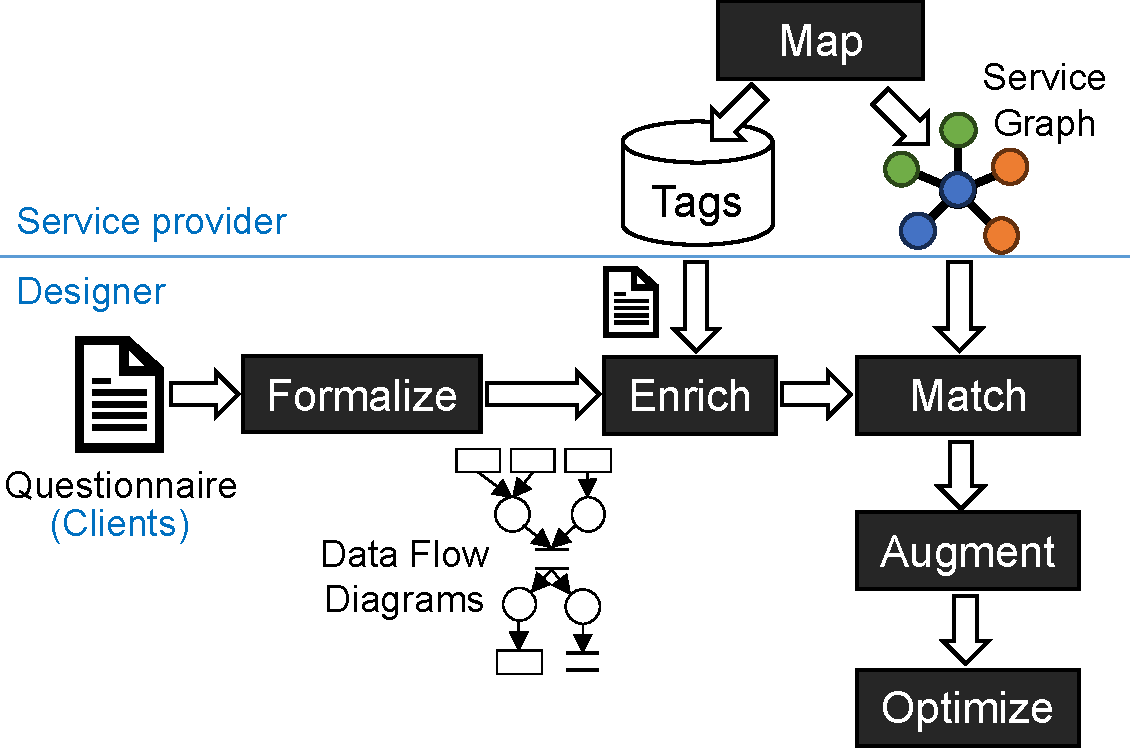
\includegraphics[width=0.8\textwidth]{parts/methods/images/overview.pdf}
    \caption{Overview of the methodology.}
    \label{fig:pdd-overview}
\end{figure}

Engineering a data platform is nontrivial. A data platform must be designed upon a principle of modularity to be extensible with new components and functionalities. While it is true that reference architectures exist (as later discussed in \Cref{sec:pdd-related}), not all their modules and services might be necessary. Indeed, running useless functionalities and services results in a waste of resources and money (e.g., in cloud environments where users pay for the running time of the allocated resources).

To effectively build a data platform, we propose a methodology (\Cref{fig:pdd-overview}) that involves three types of users: \emph{cloud service providers} (IT experts with in-depth knowledge of services available in the ecosystem); data platform \emph{designers} (consultants or people with expertise in designing data flows but with no vertical knowledge on cloud/service ecosystems) and \emph{clients} asking for the design of the data platform blueprint (e.g., partners involved in the same European project with expertise on the applicative domain ---such as precision agriculture--- but no expertise on IT and architectures). {\color{red}In the setting of this thesis, a client corresponds to the developer of a Digital Twin's user process (\Cref{sec:dataplat-refarch}): someone with expertise in the physical process or application domain the Digital Twin represents, but not necessarily in the underlying data infrastructure.}

The methodology aims to assist designers in selecting the services necessary to implement the clients' data pipelines out of the ``unstructured'' lists of services provided by cloud providers.

Here, we sketch the five steps composing the methodology, and we mainly focus on steps (4), (5), and (6) in the remainder of the chapter.

\paragraph{(1) Define the service ecosystem.}
A cloud service provider identifies \textit{una tantum}: (i) the alternative candidate services to compose the blueprints of data platforms, and (ii) a taxonomy of tags that describe and characterize such services. The identified services are organized in a service graph describing the preferences and relationships between them as well as the tags characterizing each service.

Assuming that cloud service providers do not offer redundant services, our guideline for designing the tag taxonomy emphasizes ensuring sufficient expressiveness. This means that each service should be uniquely identifiable by a set of tags.

\begin{example}
Within the Amazon Web Services (AWS) ecosystem, there are several services for managing relational data but they have different purposes. For instance, RDS is used to manage operational workloads while Redshift is used to manage data warehouses and OLAP workloads. To distinguish these two services, the tag taxonomy should be expressive enough (i.e., have enough tags) so that RDS and Redshift differ for at least one tag.
\end{example}

\paragraph{(2) Formalize the requirements through a Data Flow Diagram.}
When building the blueprint of a new data platform, clients compile questionnaires that collect information about their data-driven processes and the main steps, subjects, and goals of their analysis. Note that the data platform should support (possibly independent) processes from multiple clients.

Designers then refine the answers to the questionnaires and formalize the processes into a Data Flow Diagram (DFD); during the process, a few interviews with the clients might be necessary. We choose the DFD formalism \cite{DeMarco78} since it represents flows of data through an information system at a high level of abstraction, emphasizing the movement and transformation of data while hiding details such as decision points and interactions: knowing which repositories and processes compose the data-driven processes is enough to return a blueprint.

To build the DFD, designers decompose the data flows into agents, processes, and repositories. Starting from an aggregated overview, our guideline is to recursively split candidate processes and repositories until each of them is characterized by homogeneous tags (e.g., if a repository contains both unstructured images and relational tables, split it into two homogeneous repositories). Repositories and processes that should not be imported into the data platform (e.g., legacy systems deployed on-premises) should be treated as external agents.

\paragraph{(3) Enrich the DFD with service tags.}
To match the DFD with the services deployed in a cloud ecosystem, the two must share the same characterization. Each process and repository in the DFD is enriched with the tags from the taxonomies previously identified by the cloud service provider. To aid designers in the characterization of each process/repository (agents are not subjects of enrichment, since they are out of the scope of the platform), clients answer an additional set of questions; we recall that clients are not required to have vertical knowledge about computer and data science or engineering. Such questions are defined by the cloud service providers and driven by the tag taxonomies. Note that since our final goal is selecting the most appropriate services, we are not interested in identifying and tracking the data/processes but rather their types and their flows.

\begin{example}
Given a repository from the DFD, we ask the question: ``What are the main types of collected data?'' -- Sensor data, Images, Videos, Satellite observations, \textbf{Tables}. Answering ``Satellite observations'' tags the repository with the properties \prop{Volume}{Big}, \prop{Data Model}{File}, and \prop{Data Nature}{Raster} since earth observations are data-heavy files (e.g., around 1 GB for 100 $km^2$) and tags the process to download such data as \prop{Collection}{Pull} since files are downloaded from an FTP server \cite{esa-eo}.
\end{example}

\paragraph{(4) Match the DFD and service graphs.}
Once the DFD and service graphs are characterized by tags from the same taxonomies, it is possible to join them in a matched graph. A DFD process or repository matches (i.e., can be implemented by) a service only if the service has the same or more functionalities to fully implement it.

\paragraph{(5) Augment the matched graph.}
Augmentation is a semi-automatic step atop the matched graph. On the one hand, the system automatically recognizes architectural design patterns in the data pipelines to either automatically apply or simply highlight advanced compositions of services. On the other hand, designers can manually inject their knowledge to enrich the matched graph and steer the subsequent optimization. Designers could force the selection of services in case they are required by clients, prefer some services in place of others for performance or compatibility reasons, and refine the match (e.g., consider only services supporting programming languages required by legacy software).

\paragraph{(6) Select the optimal services.}
Out of all the services that are candidate implementations, it is necessary to select the minimal blueprint of the data platform that covers all the DFD entities (the fewer the services, the lower the cost and management efforts). Furthermore, dependencies and compatibilities between services have to be taken into account.

\subsection{Case Study: Agritech}
\label{sec:pdd-case}

Within the Agritech spoke of the NRRP European project \cite{pnrr}, we deploy a data platform supporting prescriptive analytic tasks from 8 clients in the field of precision agriculture.\footnote{{\color{red}This figure refers to the client base considered for the process-driven design methodology; \Cref{chap:dataplat} discusses the same Spoke~3 initiative with reference to its 6 formal research partners. The two counts are not necessarily inconsistent (e.g., industrial use cases versus partner institutions), but have not been independently reconciled for this thesis.}} We will use one of the partners as a working case study throughout the chapter. Here follows a qualitative description of one of the clients' data flows that the platform must support.

\begin{example}
\label{ex:pdd-qgen}
The analysis entails a flow that is structured as follows. (i) Data comes from soil moisture sensor grids, weather stations, and SENTINEL-2 satellites; (ii) Sensor and weather data is uploaded every 15 minutes to the platform, while satellite data is periodically downloaded; (iii) Soil moisture data is interpolated using mathematical (e.g., bilinear interpolation) and machine learning (e.g., neural networks) techniques; (iv) Vegetation indexes are computed out of the raw satellite observations and integrated with the enriched sensor data; (v) Reports are periodically generated out of the integrated data; (vi) Given an optimal soil moisture matrix, the integrated data is used to decide how much to irrigate the soil.
\end{example}

\begin{figure}[htbp]
    \centering
    %[FIGURE: DFD dell'esempio -- Moisture Sensors/Weather Stations -> Consume -> Sensor Data; Satellite -> Download -> Raw Images; Sensor Data -> Enrich -> Integrated Data; Raw Images -> vegetation index -> Integrated Data; Integrated Data -> ETL -> Data Warehouse; Irrigation Optimization -> Field Valves]
    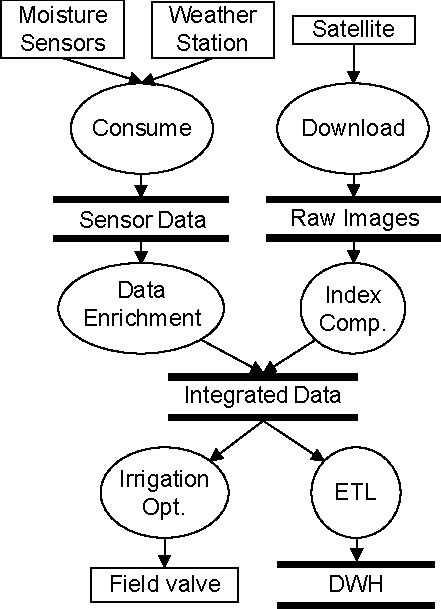
\includegraphics[width=0.4\textwidth]{parts/methods/images/dfd.pdf}
    \caption{DFD from \Cref{ex:pdd-qgen}.}
    \label{fig:pdd-dfd}
\end{figure}

After gathering questionnaires from the clients, we (designers) iteratively refined the interview into a DFD.
\begin{example}[DFD]
\Cref{fig:pdd-dfd} depicts the tasks from \Cref{ex:pdd-qgen} using the DFD formalism.
\begin{itemize}
    \item \dfd{Moisture Sensors} and \dfd{Weather Stations} stream data into the platform, such data is \dfd{Consume}d and stored in the original format into \dfd{Sensor Data};
    \item \dfd{Satellite} images are periodically \dfd{Download}ed and stored into \dfd{Raw Images};
    \item \dfd{Sensor Data} are \dfd{Enrich}ed, interpolated, and stored into \dfd{Integrated Data};
    \item \dfd{Raw Image}s are used for the computation of vegetation indexes and integrated with sensor data;
    \item \dfd{Integrated Data} are used to fuel a \dfd{Data Warehouse} through \dfd{ETL};
    \item The \dfd{Irrigation Optimization} algorithm controls the \dfd{Field Valve}s installed in Emilia Romagna, Italy.
\end{itemize}
Following the guidelines, the data collection processes cannot be merged into a single one since (i) \dfd{Moisture Sensors} streams data into the platform while \dfd{Satellite} images are periodically downloaded, and (ii) \dfd{Sensor Data} and \dfd{Raw Images} cannot be grouped into a single repository since they contain heterogeneous data types. More details on such tasks are described in \cite{DBLP:journals/cea/FranciaGG22,baldi2023smart}.
\end{example}

\subsection{Mapping the Service Ecosystem}
\label{sec:pdd-eco}

Tags (\Cref{tab:pdd-tags}) are organized as a collection of hierarchies that can be fueled bottom-up from the documentation of cloud services providers (i.e., the set of tags that are attached to each service or that are inferrable through the service description), and top-down from the literature; for instance, the big data V's \cite{anuradha2015brief}, such as volume (small to big), variety (structured to unstructured), and velocity (low to high).

\begin{definition}[Hierarchy]
A \emph{hierarchy} $h$ is a taxonomy of categorical values $Dom(h)$. $\geq_{h}$ is the partial order that defines the taxonomy; $\geq_{h}$ indicates whether a value is more specific than another. We denote with $H$ the set of hierarchies.
\end{definition}

\begin{example}[Tags and hierarchies]
\Cref{tab:pdd-tags} depicts an example of hierarchies $H=\{\sf{Data Model}, \sf{Volume}, ...\}$. In the partial order of the hierarchy $h=\sf{Data Model}$ it is, for instance, $\textup{Relational}\geq_{\sf{Data Model}} \textup{Structured} \geq_{\sf{Data Model}} \textup{Data Model (All)}$. $\textup{Relational}$ is more specific than $\textup{Structured}$ in the \sf{Data Model} hierarchy.
\end{example}

\begin{table}[!ht]
\centering
\scriptsize
\caption{Examples of taxonomies of tags.}
\label{tab:pdd-tags}
\begin{tabular}{lll}
Data Model (All)        & Structured            & Relational\\\cline{3-3}
                        &                       & Multidimensional\\\cline{2-3}
                        & Semi-structured       & Document\\\cline{3-3}
                        &                       & Wide-column\\\cline{2-3}
                        & Unstructured          & Key-value\\\cline{3-3}
                        &                       & Graph\\\cline{3-3}
                        &                       & File (text, binary)\\\cline{1-3}
&&\\
Data Nature (All)       & Spatial               & Vectorial\\\cline{3-3}
                        &                       & Raster\\\cline{2-3}
                        & Temporal              & \\\cline{1-2}
&&\\
Volume (All)            & Small                 & \\\cline{2-2}
                        & Big                   & \\\cline{1-2}
&&\\
Data Zones (All)   & Landing               & \\\cline{2-2}
                        & Archive               & \\\cline{2-2}
                        & Processed             & \\\cline{1-2}
&&\\
Functionality (All)& ETL                   & \\\cline{2-2}
                        & Reporting        & \\\cline{2-2}
                        & Operational           & \\\cline{2-3}
                        & Machine learning      & Classification\\\cline{3-3}
                        &                       & Regression\\\cline{1-3}
&&\\
Collection (All)        & Pull                  & Cumulative\\\cline{3-3}
                        &                       & Delta\\\cline{2-3}
                        & Push                  & \\\cline{1-2}
&&\\
Computing (All)         & Batch                 & \\\cline{2-2}
                        & Mini-batch            & \\\cline{2-2}
                        & Streaming             & \\\cline{1-2}
&&\\
Language (All)          & Low code              & \\\cline{2-2}
                        & Python                & \\\cline{2-2}
                        & Java                  & \\\cline{2-2}
                        & SQL                   & \\\cline{1-2}
\end{tabular}%
\end{table}%

\begin{table}[htbp]
  \centering
  \scriptsize
  \caption{An excerpt of services from the Amazon AWS ecosystem (from \url{https://aws.amazon.com/big-data/datalakes-and-analytics}).}
  \label{tab:pdd-awsserv}
    \begin{tabular}{lp{4cm}p{4cm}}
    \toprule
    Solution areas & Use cases & AWS services \\
    \midrule
    Advanced analytics & Interactive analytics & Athena \\
          & Big data processing & EMR \\
          & Data warehousing & Redshift \\
          & Real-time analytics & Managed Service for Apache Flink \\
          & Operational analytics & OpenSearch Service \\
          & Dashboards and visualizations & QuickSight \\
          & Visual data preparation & Glue DataBrew \\
    Data management & Real-time data movement & Managed Streaming for Apache Kafka, Kinesis Data Streams, Glue \\
          & Data governance & DataZone, Glue, Entity Resolution, Lake Formation, S3 \\
          & Object storage for data lakes & S3, Lake Formation \\
          & Backup and archive for data lakes & S3 Glacier, Backup \\
          & Data catalog & Glue, Lake Formation \\
          & Third-party data & Data Exchange, Clean Rooms \\
    Machine learning & Frameworks and interfaces & Deep Learning AMIs \\
          & Platform services & SageMaker \\
    \bottomrule
    \end{tabular}%
\end{table}%

The services available on a specific ecosystem differ for each provider, and no single and shared organization of services is available. \Cref{tab:pdd-awsserv} shows an example of services from the AWS website (as of November 2023).

While a plethora of services is available, there is no necessity to consider all of them at once. Indeed, the considered services must cover the ``core'' functionalities necessary to run a data platform such as the ones proposed by NIST \cite{chang2019nist}, among them storage and data processing engines.

Also, it is necessary to consider the relationships between services (e.g., whether the adoption of a service requires another) and preferences in their choice (e.g., due to differences in performance reasons). That is why we map the services into a directed property graph.

\begin{definition}[Directed property graph]
\label{def:pdd-graph}
A \emph{directed property graph} is a tuple $G = (N, A, P, L)$ where $N=\{..., n_i, ...\}$ is a finite set of \emph{nodes}, $A=\{..., a_{ij}, ...\}$ is a finite set of \emph{arcs} connecting nodes $n_i$ and $n_j$, $P=\{..., (h, v), ...\}$ is a set of key-value \emph{properties} with $h \in H$ and $v \in Dom(h)$, and $L$ is a set of \emph{labels}. $props: (N \cup A) \rightarrow P$ returns the properties of a node or arc. $label: (N \cup A) \rightarrow L$ returns the labels of a node or arc.
\end{definition}

\begin{definition}[Path]
Given a directed property graph $G$, a \emph{path} $p_{ij}$ from node $n_i$ to node $n_j$ is a sequence of distinct arcs $(a^1_{ix}, ..., a^k_{xy}, ..., a^{|p|}_{yj})$ for which there is a sequence of distinct nodes $(n^1_{i}, ..., n^k_{x}, n^{k+1}_{y}, ..., n^{|p|+1}_{j})$ such that the arc $a^k$ connects the node $n^k$ to the node $n^{k+1}$ for $k \in [1, |p|]$. We denote with $p_{ij}.nodes$ the sequence of nodes connected by the path.
\end{definition}

\begin{figure}[htbp]
    \centering
    %[FIGURE: excerpt di service graph -- nodi S3, GeoServer, EC2, EMR, Lakehouse con archi Requires/IsCompatible e relative property]
    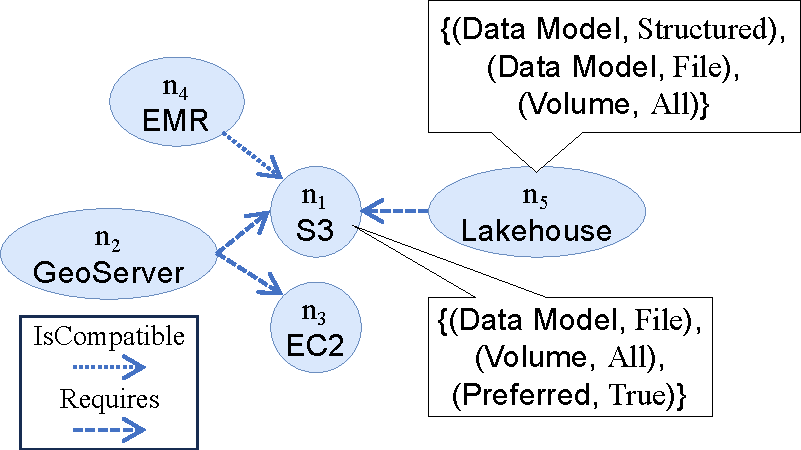
\includegraphics[width=0.7\textwidth]{parts/methods/images/servicegraph.pdf}
    \caption{Excerpt of a service graph and its properties.}
    \label{fig:pdd-servicegraph}
\end{figure}

\begin{definition}[Service graph]
\label{def:pdd-serv}
A \emph{service graph} is a directed property graph $G^S$ where nodes are labeled as \lbl{Service}, while arcs are alternatively labeled as $\{\lbl{Requires}, \lbl{IsCompatible}, \lbl{IsAkin}\}$.
\end{definition}

The semantics of the labels is the following:
\begin{itemize}
    \item \lbl{Service}: is any engine from the service ecosystem that can be optionally tagged with the property \prop{Preferred}{True} to specify whether it should be considered more than others;
    \item \lbl{Requires}: represents whether a service mandatorily relies on another;
    \item \lbl{IsCompatible}: represents whether a service natively interfaces with another (i.e., their interaction is supported by default and does not require custom/additional libraries or connectors);
    \item \lbl{IsAkin}: represents whether a service not only is compatible with another but also if their adoption together is encouraged.
\end{itemize}

\begin{example}[Service graph]
Here follows an excerpt of the service graph $G^S$ and properties built out of \Cref{tab:pdd-awsserv} and depicted in \Cref{fig:pdd-servicegraph}.
\begin{align*}
&N = \{n_1, n_2, n_3, n_4, n_5,...\}, ~
A =\{a_{23}, a_{34}, ...\}\\
&n_1 = \serv{S3},~n_2=\serv{GeoServer},~n_3=\serv{EC2},~n_4=\serv{EMR}
,~n_5 = \serv{Lakehouse}
\\
&label(n_1) = \lbl{Service}\\
&label(a_{23}) = \lbl{Requires}\\
&label(a_{41}) = \lbl{IsCompatible}\\
&props(n_1) = \{\prop{Data Model}{File},\prop{Volume}{All}, \prop{Preferred}{True}\}\\
&props(n_2) = \{\prop{Data Model}{File},\prop{Data Nature}{Raster}\}\\
&
props(n_5)=\{\prop{Data Model}{Structured},\prop{Data Model}{File},\prop{Volume}{All}\}
\end{align*}
\serv{GeoServer} requires \serv{EC2} since it is deployed on it, \serv{EMR} is compatible with \serv{S3} since it can natively read from and write to the object storage.
\end{example}

\subsection{Process-Driven Match, Augmentation, and Optimization}
\label{sec:pdd-process}

We now describe three steps composing our approach. \textit{Match} extracts the services that can support the execution of the data pipeline, \textit{Augment} refines the potential candidates and, finally, \textit{Optimize} picks the optimal (minimal) subset. We mainly focus on the optimization of the platform design rather than on how, starting from questionnaires, designers refine the DFD of such flows.

Since data pipelines are the backbone of data platforms, everything starts from the DFD describing the processes of clients' analysis.

\begin{definition}[Data Flow Diagram]
\label{def:pdd-dfd}
A \emph{Data Flow Diagram} (DFD) is a directed property graph $G^D$ where nodes are alternatively labeled as $\{\lbl{Agent}, \lbl{Repository}, \lbl{Process}\}$, while arcs are labeled as \lbl{Flow}. Arcs must connect with at least one node with label \lbl{Process}. The semantics of the labels is the following:
\begin{itemize}
    \item \lbl{Agent}: an external entity that communicates with the system and stands outside of the system;
    \item \lbl{Process}: transform inputs to outputs;
    \item \lbl{Repository}: store data for later use;
    \item \lbl{Flow}: transfer data from one part of the system to another.
\end{itemize}
\end{definition}

We recall that the DFD is enriched with tags identified by the cloud service provider (\Cref{tab:pdd-tags}).

\begin{figure}[htbp]
    \centering
    %[FIGURE: excerpt di property del DFD -- nodo Consume (Process) con archi verso Sensor Data (Relational) e Raw Images (File, Raster)]
    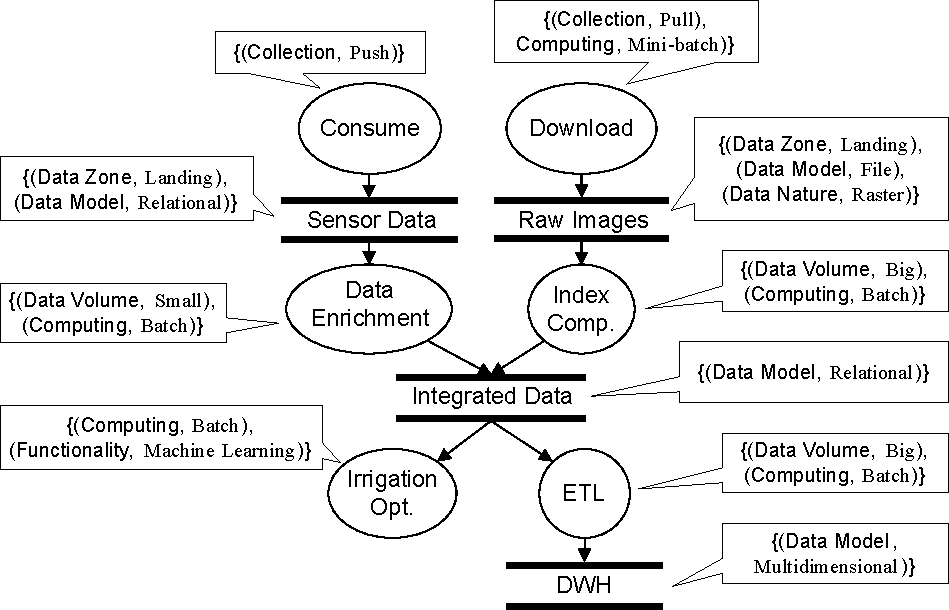
\includegraphics[width=0.8\textwidth]{parts/methods/images/dfd-ext.pdf}
    \caption{An excerpt of properties of the DFD from \Cref{fig:pdd-dfd}.}
    \label{fig:pdd-dfd-ext}
\end{figure}

\begin{example}[DFD]
Here follows an excerpt of the DFD $G^D$ and properties from \Cref{fig:pdd-dfd-ext}.
\begin{align*}
&N = \{n_1, n_2, n_3, ...\},~A =\{a_{12}, ...\}\\
&n_1 = \dfd{Consume},~n_2=\dfd{Sensor Data},~n_3=\dfd{Raw Images}\\
&label(n_1)= \lbl{Process},~label(n_2)= \lbl{Repository}\\
&label(n_3)= \lbl{Repository},~label(a_{12})=\lbl{Flow}\\
&props(n_2)= \{\prop{Data Model}{Relational}\}\\
&props(n_3)= \{\prop{Data Model}{File}, \prop{Data Nature}{Raster}\}
\end{align*}
\end{example}

\subsubsection{Matching the DFD and Service Graphs}

Given the service graph and the DFD, we can automatically join them by matching their tags.

\begin{definition}[Match]
\label{def:pdd-nodematch}
Given a DFD and a service graph, the function $match: N^D \times N^S \rightarrow \{true, false\}$ is true when, given a node $n^D \in N^D$ of the DFD and a node $n^S \in N^s$ of the service graph, each property in $props(n^D)$ matches a property in $props(n^S)$. A property $(h_i,v_i)$ matches another property $(h_j, v_j)$ if $h_i=h_j$ and $v_i \geq_{h_i} v_j$.
\end{definition}

A match represents whether a DFD node can be implemented using a specific service (solid arcs in \Cref{fig:pdd-match}); i.e., services that have the same or more generic values for the properties specified in the DFD node. For instance, a DFD repository tagged as Relational could be implemented by services supporting Relational or all Structured data.

\begin{example}[Match]
With reference to \Cref{fig:pdd-match}, given the node \dfd{Raw Images} from the DFD, and the nodes \serv{S3} and \serv{GeoServer} from the service graph
\begin{align*}
props(\dfd{Raw Images}) &= \{\prop{Data Model}{File},\prop{Data Nature}{Raster}\}\\
props(\serv{GeoServer}) &= \{\prop{Data Model}{File},\prop{Data Nature}{Raster}\}\\
props(\serv{S3}) &= \{\prop{Data Model}{File},\prop{Volume}{All}\}
\end{align*}
Since $match(\dfd{Raw Images}, \serv{GeoServer}) = true$ and $match(\dfd{Raw Images}, \serv{S3}) = false$, \dfd{Raw Images} can be implemented by \serv{GeoServer} but not directly in \serv{S3}. The former is natively capable of managing geographical data while \serv{S3} would only provide storage as plain files.
\end{example}

\begin{figure}[htbp]
    \centering
    %[FIGURE: matching tra grafo DFD (bianco) e grafo servizi (blu); in grassetto i servizi selezionati come blueprint ottimale; Athena e Churn Prediction come esempi di servizi non abbinati]
    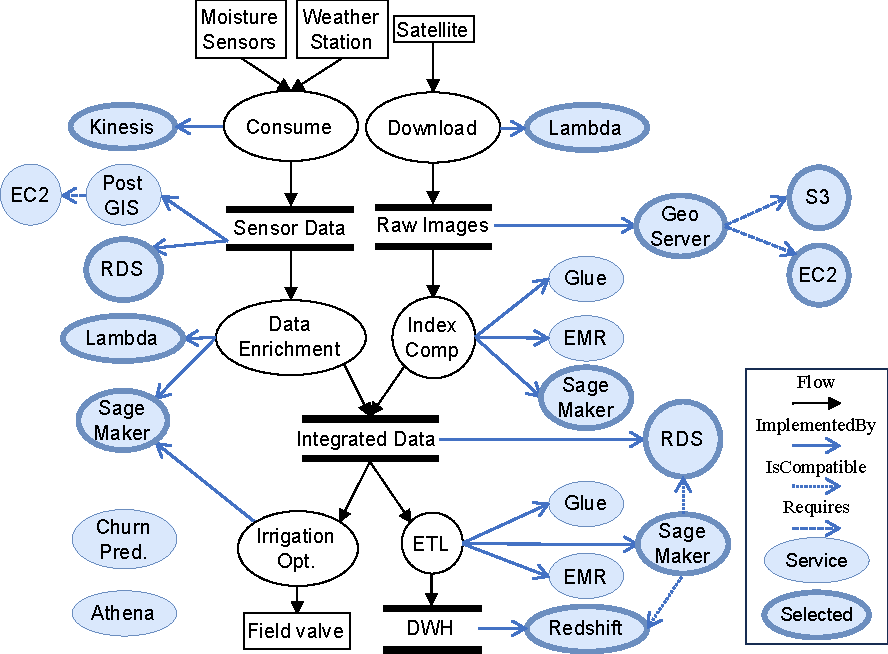
\includegraphics[width=0.75\textwidth]{parts/methods/images/graph.pdf}
    \caption{Matching the DFD (white) and service (blue) graphs; in bold the services selected as the optimal blueprint for the data platform design. \serv{Athena} and \serv{Churn Prediction} are examples of unmatched services that are available in the AWS ecosystem.}
    \label{fig:pdd-match}
\end{figure}

\begin{definition}[Matched graph]
\label{def:pdd-match}
Given a DFD $G^D = (N^D, A^D, P^D, L^D)$ and a service graph $G^S = (N^S, A^S, P^S, L^S)$, a matched graph $G^M = (N^D \cup N^S, A^D \cup A^S \cup A, P^D \cup P^S, L^D \cup L^S \cup \{\lbl{ImplementedBy}\})$ is a directed property graph obtained as the union of $G^S$ and $G^D$. $A$ is an additional set of arcs, one for every match between nodes in $N^S$ and $N^D$. Arcs in $A$ are labeled as \lbl{ImplementedBy} and can have an optional property \prop{Mandatory}{True} to specify that such implementation must be selected in the final blueprint.
\end{definition}

The result of a match is a graph that is composed of the union of the nodes, and the union of the arcs plus additional arcs that represent candidate implementations for the DFD processes/repositories. The label \lbl{ImplementedBy} represents whether a DFD process or repository can be implemented by a specific service. If no match is found for a DFD node, we alert the designer in order to verify that the DFD has been properly designed and/or enriched with the service tags.

\begin{example}[Matched graph]
\Cref{fig:pdd-match} depicts an excerpt of the matched graphs for the DFD from \Cref{fig:pdd-dfd}; for the sake of clarity, not all the arcs have been presented. Nodes from the DFD have a white background, while services are represented in blue. Solid arrows represent arcs labeled as \lbl{ImplementedBy} (e.g., \dfd{Sensor Data} can be implemented by either \serv{PostGIS} or \serv{RDS}). Dotted arrows represent arcs labeled as \lbl{IsCompatible} (e.g., \serv{SageMaker} reads from and writes to \serv{Redshift}). Dashed arrows represent arcs labeled as \lbl{Require} (e.g., \serv{GeoServer} requires \serv{EC2} since it is deployed on it). Of course, it is unlikely that all services of the cloud ecosystem will be matched; \serv{Athena} and \serv{Churn Prediction} are examples of unmatched services.
\end{example}

\subsubsection{Augmenting and Pruning the Matched Graph}

Designing a platform is not just a technical task but encompasses various organizational, business, and political aspects that must be carefully considered. The successful creation of a platform requires the expertise and experience of designers to manipulate the matched graph and aid in the subsequent optimization. This ensures that the platform is not only technically sound but also aligns with broader strategic goals and user needs.

In our approach, designers have several tools at their disposal to influence and refine the design process:
\begin{itemize}
    \item Force the selection of specific services: designers can mandate the inclusion of certain services due to various factors such as client requirements, industry standards, or established design practices. This is accomplished by adding the property \prop{Mandatory}{True} to \lbl{ImplementedBy} arcs in the matched graph. By doing so, designers ensure that essential services are incorporated into the platform.
    \item Prefer certain services over others: in many cases, some services are more desirable than others due to their superior efficiency, reliability, or user familiarity. Designers can indicate these preferences by adding the property \prop{Preferred}{True} to the nodes labeled as \lbl{Service} in the matched graph. This preference can optimize the platform's blueprint and user experience by prioritizing the most advantageous services.
    \item Refine the match: designers can fine-tune the matched graph by preliminarily removing services that do not meet specific criteria or adding services that were initially unmatched. For example, they might exclude services that do not support required programming languages for legacy software or add missing matches due to incomplete tagging. This refinement ensures the platform is both relevant and comprehensive, accommodating all necessary components and integrations.
\end{itemize}

\begin{example}[Mandatory and preferred services]
With reference to \Cref{fig:pdd-match}, imagining that our methodology is used to lift-and-shift an on-premises solution that already used \serv{GeoServer} to AWS, \serv{GeoServer} could be tagged with the property $\prop{Mandatory}{True}$ since clients already have experience with it (and not with alternative engines such as \serv{GoogleEarth}). Also, since \serv{S3} is cheaper than other storage services (such as \serv{EBS} and \serv{EFS}), \serv{S3} could be tagged with the property $\prop{Preferred}{True}$.
\end{example}

After manual adjustments, an automated pruning process removes sub-graphs that are not reachable from the DFD. These sub-graphs represent services that are neither candidate implementations nor accessible from candidate implementations.

\begin{example}[Pruning the matched graph]
In \Cref{fig:pdd-match}, \serv{Churn Prediction} and \serv{Athena} are discarded before the optimization since they are not reachable from any DFD entity (i.e., they are neither candidate implementations nor required by other services).
\end{example}

Finally, this step supports the recognition, matching, and refinement of design patterns, as discussed in \Cref{sec:pdd-patterns}. Design patterns ensure that the data platforms adhere to best practices and maintain a high standard of quality and maintainability.

\subsubsection{Optimizing the Blueprint}
\label{ssec:pdd-opt}

The optimization of the services comprising a data platform can take various forms, depending on the numerous influencing factors and the diverse objectives of clients, such as cost reduction, simplified management, or enhanced extensibility. In this chapter, we use the minimization of the number of services as an objective function since this indicator correlates with both cost minimization and management simplicity. It will be seen later that other desirable properties of the chosen solution (e.g., adherence to business practices and compatibility with other systems already present in the company) can be easily satisfied through the preferences indicated by users.

However, such optimization is not trivial. For instance, some DFD entities can be implemented atop alternative services (e.g., a data lake that is implemented either on \serv{S3} or \serv{HDFS}), and some services are meaningful only if they cover at least two DFD entities (e.g., we use a \serv{Lakehouse} to replace both a data lake and a data warehouse). The selection must be compliant with the following conditions.
\begin{itemize}
    \item \textit{Coverage}: all processes and repositories in the DFD must be covered.
    \item \textit{Dependency}: if a service is selected, all its required services must be (recursively) selected too (e.g., \serv{Geoserver} is deployed on \serv{EC2}).
    \item \textit{Compatibility}: a service can be selected only if it is compatible with the services selected for the previous (if existing) and following (if existing) nodes in the DFD.
    \item \textit{Preference}: services marked as preferred should have more chances to be selected (for instance, preferences can be expressed for services entailing lower costs or higher performance).
    \item \textit{Mandatory}: service implementations marked as mandatory must be selected for the blueprint (e.g., a certain repository must be implemented by a document-based service).
    \item \textit{Affinity}: if a service is selected, services with high affinity should be selected too.
\end{itemize}

\begin{figure}[htbp]
{\footnotesize
\begin{align}
&min \sum_i w_i s_i \textup{ such that }\\
&s_i \in \{0,1\} \textup{ for all } n_i \in N, label(n_i) = \lbl{Service}\\
&s_{ij} \in \{0,1\} \textup{ for all } a_{ij} \in A, label(a_{ij})= \lbl{ImplementedBy}\\
&s_j \geq s_{ij} \textup{ for all } s_{ij}\\
&\sum_{a_{ij} \in A, label(a_{ij})=\lbl{ImplementedBy}} s_{ij}=1  \textup{ for all } n_i \in N, label(n_i) \in \{\lbl{Process}, \lbl{Repository}\}\\
&s_j\geq s_i  \textup{ for all } a_{ij} \in A, label(a_{ij})= \lbl{Requires} \\
&s_{ij}+s_{kh} \leq 1  \textup{ for all } a_{ik} \in A, a_{jh} \notin A, label(a_{ik})=\lbl{Flow}, label(a_{jh})=\lbl{IsCompatible}\\
&s_{ij} = 1 \textup{ for all } a_{ij} \in A, \prop{Mandatory}{True} \in props(a_{ij})\\
&s_{ij} \cdot s_{kh} \geq s_{h} \textup{ for all } a_{ik}, a_{jh} \in A, label(a_{ik})=\lbl{Flow}, label(a_{jh})=\lbl{IsAkin}
\end{align}
}
\caption{Selecting the optimal services considering coverage (5), dependency (6), compatibility (7), and mandatory (8), and affinity (9) constraints.}
\label{fig:pdd-form}
\end{figure}

More formally, given a matched graph $G^M=(N, A, P, L)$, the selection of the optimal blueprint can be modeled as a linear programming problem inspired by the standard \emph{facility location problem}. In a basic formulation, the facility location problem consists of a set of potential facility sites where a facility can be opened, and a set of demand points that must be serviced. The goal is to pick a subset of facilities to open while minimizing the sum of distances from each demand point to its nearest facility plus the sum of opening costs of the facilities. In our case, services are mapped to the potential locations while DFD nodes are mapped to the demand points. The formulation in \Cref{fig:pdd-form} reads as follows.
\begin{itemize}
    \item[(1)] The optimization function minimizes the weighted sum of the selected services. Weights $w_i$ specify preferences for services $s_i$, we set
    \[
    w_i=\begin{cases}
    0.5 & \textup{if } \prop{Preferred}{True} \in props(n_i)\\
    1.0 & \textup{otherwise}
    \end{cases}
    \]
    In case multiple optimal solutions exist, we return all of them to the designers so that they can compare them and select the one they find the most appropriate since there is no solution dominating the others. When no solution is feasible (e.g., due to a lack of matches or incompatibility of mandatory services) the system alerts the designers since a refinement of the DFD could be necessary.
    \item[(2)] $s_i$ are binary variables modeling services. $s_i=1$ if the service is selected, $0$ otherwise.
    \item[(3)] $s_{ij}$ are binary variables modeling the services implementing DFD processes and repositories. $s_{ij}=1$ if $n_i \in N$ s.t. $label(n_i) \in \{\lbl{Repository}, \lbl{Process}\}$ is implemented by $n_j \in N$ s.t. $label(n_j) = \lbl{Service}$.
    \item[(4)] Binding variables $s_j$ and $s_{ij}$: service $s_j$ is selected if it implements ($s_{ij}=1$) a DFD node $n_i \in N$ s.t. $label(n_i) \in \{\lbl{Repository}, \lbl{Process}\}$.
    \item[(5)] \emph{Coverage} constraints: every repository and process must be implemented by exactly one service.
    \item[(6)] \emph{Dependency} constraints: if a service is selected, all the services it depends on must be selected.
    \item[(7)] \emph{Compatibility} constraints: if two services are incompatible, they cannot be selected to implement two consecutive processes/repositories linked through a data flow in the DFD.
    \item[(8)] \emph{Mandatory} constraints: if an implementation is mandatory and tagged with the property \prop{Mandatory}{True}, $s_{ij}$ is set to 1.
    \item[(9)] \emph{Affinity} constraints: if the service $s_h$ is selected and has affinity with another service $s_j$, then $s_j$ is selected too.
\end{itemize}

\begin{example}[Optimization]
\label{ex:pdd-optimization}
Given the matched graph from \Cref{fig:pdd-match}, the \textit{optimal} blueprint of the data platform is represented by the services highlighted in bold (with a cost of 7.5), namely \serv{Kinesis}, \serv{Lambda}, \serv{RDS}, \serv{EC2}, \serv{SageMaker}, \serv{GeoServer}, \serv{S3} (tagged as preferred), and \serv{Redshift}. \serv{GeoServer} has been selected since it is the only available implementation for \dfd{Raw Images}, \serv{EC2} and \serv{S3} have been selected since they are required by \serv{GeoServer}. \serv{SageMaker} has been selected and preferred to \serv{EMR} and \serv{Glue} since three DFD processes can be implemented on it.
\end{example}

\subsection{Design Patterns}
\label{sec:pdd-patterns}

Clients' data pipelines could present \textit{design patterns} (i.e., solutions to common problems in software and architecture design) that require certain constraints to be satisfied on the overall data pipeline (and not only on single nodes in the DFD and their properties). Design patterns are important since they impact the services that are matched and selected for the optimal blueprint.

\subsubsection{Defining Design Patterns}

Design patterns are retrieved from the DFD graph.
\begin{definition}[Architectural Design Pattern]
Given a DFD graph $G^D$, a design pattern $p$ is a subgraph $\bar{G} \in G^D$ in which $cond_p(\bar{G})$ holds. $cond_p(\bar{G})$ is specific to each design pattern and can be expressed in terms of graph queries on the DFD graph.
\end{definition}

Since our definition of design pattern is ``generic'', design patterns could impact our approach in different ways. The simple recognition of design patterns could already be informative for the designer of the data platform (the recognition of the pattern itself could help to refine the design of the platform). Additionally, patterns could alter the matched graph (by matching additional services) and the optimization procedure (by preferring some services to others). We show the impact of design patterns with reference to the \textit{Lakehouse} and \textit{Lambda Architecture} (although other patterns exist, such as the kappa architecture and the 2- or 3-layered architecture for data warehousing).

\paragraph{Lakehouse.} Lakehouse (\Cref{fig:pdd-matchlake}) is a data management paradigm that combines the capabilities of data lakes and data warehouses, enabling business intelligence and machine learning on the same data. A Lakehouse can be applied if, within the same data pipeline, there is a sequence of ETL steps that moves data from a data lake to a data warehouse, optionally passing through relational databases. Lakehouse encourages the adoption of a medallion architecture (a data design pattern)\footnote{\url{https://www.databricks.com/glossary/medallion-architecture}} where raw data is initially stored in a data lake (bronze layer), refined data are stored in a relational engine (silver layer), and data cubes are stored in a multidimensional engine (gold layer). However, to avoid the additional usage of a relational engine (which would bring higher costs and effort into keeping the 3 layers aligned), ETL could skip the intermediate storage and upload data directly into the data warehouse for simpler architectures.

Formally, a Lakehouse is a graph $\bar{G}$ with a set of nodes $\bar{N}=\{n_i, ..., n_k, ..., n_j\}$ such that $cond_{Lakehouse}(\bar{G})$ is defined as
\begin{align*}
&\exists p_{ij} ~ s.t. ~ label(n_i) = Repository \wedge \prop{Functionality}{Landing} \in prop(n_i) \wedge\\
&\qquad\qquad            label(n_j) = Repository \wedge \prop{Data Model}{Multidimensional} \in prop(n_j)
\end{align*}
and (optionally) $n_k \in p_{ij}.nodes ~ s.t. ~ \prop{Data Model}{Structured} \in prop(n_k)$. Intuitively, $n_i$ is the data lake, $n_j$ the data warehouse, and $n_k$ the optional intermediate relational storage.

\paragraph{Lambda Architecture.} Lambda architecture (\Cref{fig:pdd-lambda}) is a data-processing architecture designed to handle massive quantities of data by taking advantage of both batch and stream processing. It uses batch processing to provide comprehensive and accurate views of batch data, while simultaneously using real-time stream processing to provide views of online data. Formally, a Lambda architecture is a graph $\bar{G}$ with a set of nodes $\bar{N}=\{n_i, n_j, n_k, n_l\}$ such that $cond_{Lambda}(\bar{G})$ is defined as the conjunction of the following conditions
\begin{align*}
&\exists p_{ij} ~ s.t. ~ label(n_i) = Process \wedge \prop{Collection}{Push} \in prop(n_i) \wedge\\
&\qquad\qquad label(n_j) = Process \wedge \prop{Computing}{Streaming} \in prop(n_j),\\
&\exists p_{ik} ~ s.t. ~ label(n_k) = Repository \wedge \prop{Volume}{Big} \in prop(n_k),\\
&\exists p_{kl} ~ s.t. ~ label(n_l) = Process \wedge \prop{Computing}{Batch} \in prop(n_l)
\end{align*}

\subsubsection{Exploiting the Matched Graph}

Design patterns can be highlighted to designers for further evaluation or match additional services. For instance, new matches are added when design patterns can be directly implemented by services from the service graph. This is the case for Lakehouse, where a single service fulfills the requirements of an entire pattern.

\begin{figure}[htbp]
\centering
%[FIGURE: matching del pattern Lakehouse -- in grigio i processi non rilevanti, in rosso la property che impedisce il match tra Raw Images e Lakehouse]
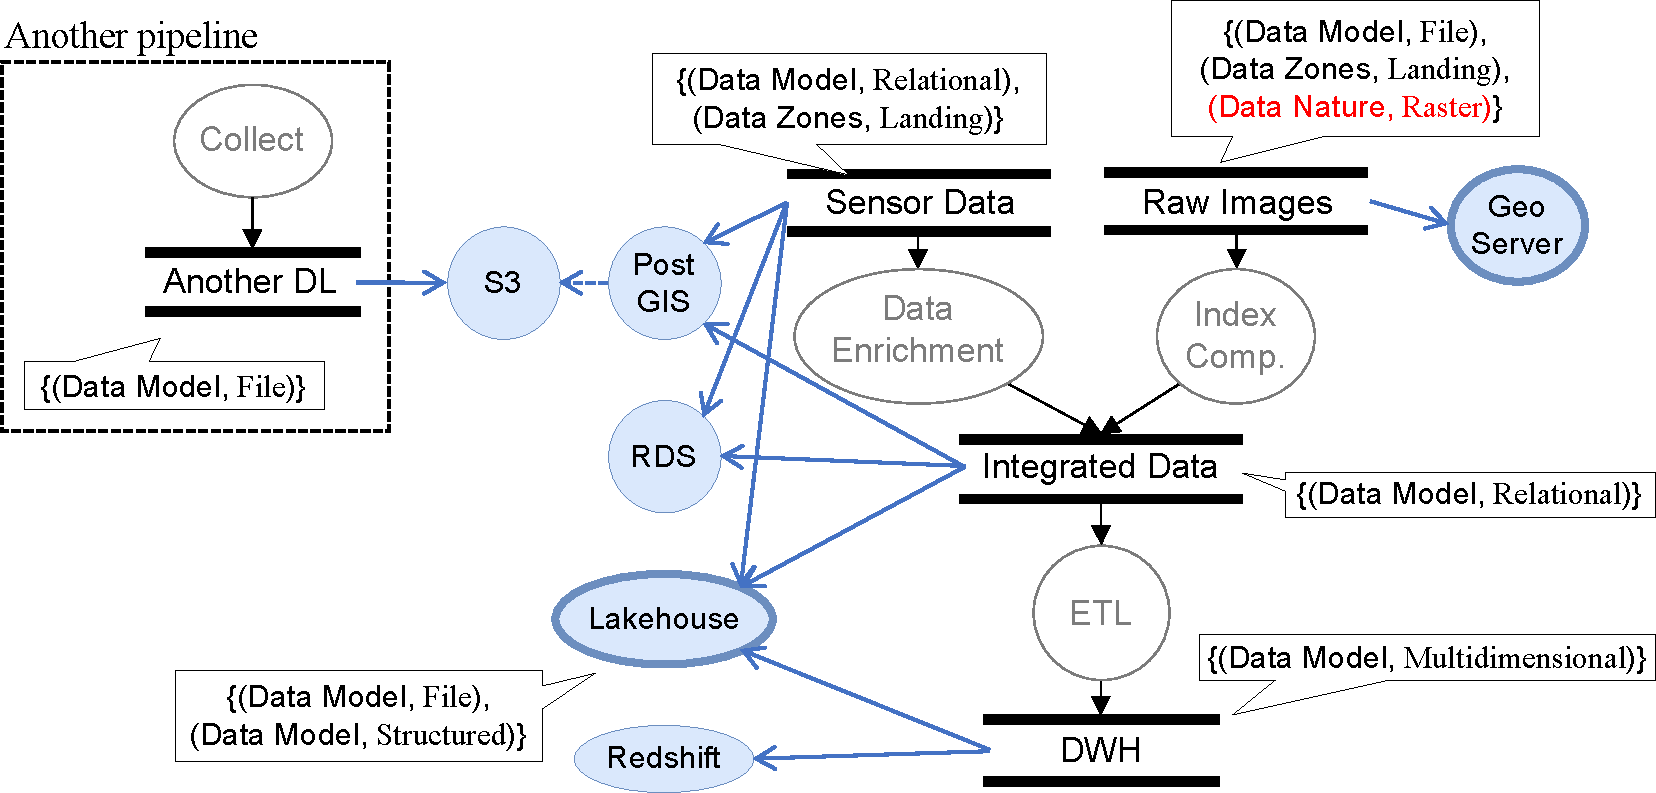
\includegraphics[width=0.8\textwidth]{parts/methods/images/matchingdl.pdf}
\caption{Matching the Lakehouse pattern; in gray the processes that are not relevant for matching the Lakehouse pattern and in red the property preventing the match between \dfd{Raw Images} and \serv{Lakehouse}.}
\label{fig:pdd-matchlake}
\end{figure}

\paragraph{Lakehouse.}

Databricks' \serv{Lakehouse} is a multi-platform service that implements the Lakehouse pattern. Given a DFD graph including one (or more) Lakehouse pattern $\bar{G}$ with nodes $\bar{N}$ and a service graph including the node $n_s=\serv{Lakehouse}$, the matched graph $G^M$ is augmented with new arcs $(N^M, A^M \cup A, P^M, L^M)$ where $A = \{a_{is} ~s.t.~ match(n_i, n_s) = true, n_i \in \bar{N}\}$ is an additional set of arcs, one for every (property) match between nodes in $\bar{N}$ and $n_s$. Arcs in $A$ are labeled as \lbl{ImplementedBy}.

In other words, the Lakehouse is a potential implementation for the DFD repositories in the path connecting a data lake to a data warehouse.

\begin{example}[Design pattern match]
\Cref{fig:pdd-matchlake} depicts two examples of matching the service \serv{Lakehouse} (processes are grayed out since they are not relevant for matching the Lakehouse pattern). \serv{Lakehouse} does not match \dfd{Another DL} since the latter belongs to a pipeline without a data warehouse. Conversely, \serv{Lakehouse} matches \dfd{Sensor Data}, \dfd{Integrated Data}, and \dfd{DWH} since in the DFD graph exists a path connecting a landing area (\dfd{Sensor Data}) to a data warehouse (\dfd{DWH}) and optionally passing through a relational repository (\dfd{Integrated Data}). In other words, this data pipeline is organized according to the medallion architecture that can be implemented by \serv{Lakehouse}. Additionally, \serv{Lakehouse} does not match \dfd{Raw Images} since it has the property \prop{Data Nature}{Raster} and \serv{Lakehouse} cannot directly manage spatial data/queries (more formally $match(\dfd{Raw Images}, \serv{Lakehouse}) = false$). Noticeably, if \serv{Lakehouse} is matched and later selected in place of \serv{RDS} and \serv{Redshift}, the cost of the solution in \Cref{ex:pdd-optimization} and \Cref{fig:pdd-match} decreases from 7.5 to 6.5.
\end{example}

\paragraph{Lambda Architecture.}
The lambda architecture does not require any augmentation since the composition of the services necessary for its implementation is already matched through the properties of single nodes. However, as we will see immediately below, its exploitation is accomplished by a modified formulation of the optimization problem.

\begin{figure}[htbp]
\centering
%[FIGURE: pattern Lambda architecture -- sorgente streaming/processing streaming, big data storage, big data batch engine]
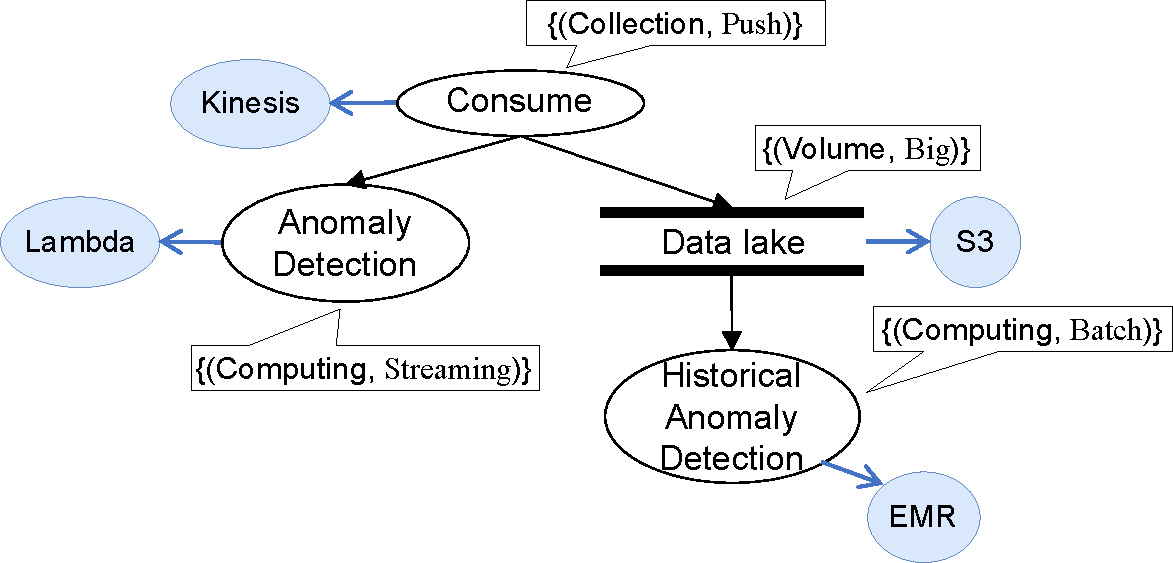
\includegraphics[width=0.7\textwidth]{parts/methods/images/lambda.pdf}
\caption{Lambda pattern.}
\label{fig:pdd-lambda}
\end{figure}

\subsubsection{Refining the Optimization}

To implement the design patterns, additional constraints could be plugged into the optimization or the weights of some services could be adjusted to prefer the adoption of some services to others.

\paragraph{Lakehouse.}

The adoption of the Lakehouse pattern $\bar{G}$ with nodes $\bar{N}=\{n_i,...,n_k,...,n_j\}$ (with $n_i$ representing a data lake, $n_j$ representing a data warehouse, and $n_k$ is an optional structured repository in between the data lake and the data warehouse) requires that, if \serv{Lakehouse} service $n_s$ is picked (i.e., $s_s=1$), such service must cover the data lake and the data warehouse as well as the optional intermediate structured repositories (there is no point in having a partial implementation of a \serv{Lakehouse}).
{\footnotesize
\begin{align*}
s_{is}\cdot ... \cdot s_{ks} \cdot ... \cdot s_{js} > s_s   \textup{ for all }& a_{is}, a_{ks}, a_{js} \in A,\\
& label(a_{is})=label(a_{ks})=label(a_{js})=\lbl{ImplementedBy}
\end{align*}
}

\paragraph{Lambda Architecture.}

The adoption of the Lambda architecture $\bar{G}$ with nodes $\bar{N}=\{n_i,n_j,n_k,n_l\}$ (with $n_i$ representing a streaming source, $n_j$ a streaming processing, $n_k$ a big data storage, and $n_l$ a big data engine) does not require additional constraints but pushes towards the adoption of some services. For instance, the AWS documentation usually leverages \serv{S3} as a big data storage, \serv{EMR} as a big data engine, \serv{Kinesis} as a streaming source, and \serv{Lambda} as streaming processing (although different services could be used, such as queuing services in place of \serv{Kinesis}). Since these services are \textit{recommended} by AWS to create a Lambda Architecture, their properties are extended with the additional property $\prop{Preferred}{True}$.
\begin{align*}
&props(\serv{S3}) = \{\prop{Preferred}{True}\} \cup props(\serv{S3})\\
&props(\serv{EMR}) = \{\prop{Preferred}{True}\} \cup props(\serv{EMR})\\
&props(\serv{Kinesis}) = \{\prop{Preferred}{True}\} \cup props(\serv{Kinesis})\\
&props(\serv{Lambda}) = \prop{Preferred}{True} \cup props(\serv{Lambda})
\end{align*}
Given the optimization problem formulated in \Cref{ssec:pdd-opt}, from Line (1) it follows that $w_i = 0.5 \textup{ if } s_i \in \{\serv{S3}, \serv{EMR}, \serv{Kinesis}, \serv{Lambda}\}$ since $w_i$ is set to 0.5 if $\prop{Preferred}{True} \in props(s_i)$. In other words, weights are decreased to 0.5 to bias the optimization towards the selection of the four services.

\subsection{Evaluation}
\label{sec:pdd-eval}

We implemented our approach (available at \url{https://github.com/big-unibo/DataPlatformDesign}) using GraphDB (to store the taxonomy of tags, the service graph, and the DFD diagrams) and Python, where we leverage the CPlex library to solve the optimization problem.

\subsubsection{Validation with Real Use Cases}
\label{sec:pdd-val}

To assess the approach, we applied it in two real contexts\footnote{We anonymize the names of the companies due to non-disclosure agreements.}: Company1 (one of the largest Italian consulting firms specialized in data analysis and with strong expertise in the field of data platforms and cloud computing) and Company2 (an international company leading in the production of smart and digitalized sports equipment). In particular, (i) we asked their experts for two use cases of data platforms implemented on different cloud service providers to prove the portability of our approach, (ii) we generated a blueprint for each use case, (iii) we asked the experts to evaluate and compare our blueprints against the ones they implemented.

In this experimental setup, we act as platform designers, whereas experts from the companies act as clients. The collection of the case studies was done by setting up 2 to 3 interviews of a maximum of 1 hour each and according to the methodology from \Cref{sec:pdd-overview}.

\begin{itemize}
    \item Step (1): we created the service graphs for Microsoft Azure and Google Cloud. We adopted the taxonomy of tags summarized in \Cref{tab:pdd-tags}.
    \item Step (2): the first interview was devoted to understanding the proposed data-driven processes: the main steps, subjects, and analysis goals. The output of the interview was the DFD diagram of the processes.
    \item Steps (3) and (4): we enriched the DFD with tags from our taxonomy and matched it with the service graphs.
    \item Step (5): the second interview was devoted to refining the DFD and augmenting the matched graph with the clients. This additional iteration on the DFD is necessary in case of ambiguities in the tagging.
    \item Step (6): we generated the blueprint and used the final interview to discuss the solution with the clients.
\end{itemize}

\begin{figure}[htbp]
    \centering
    %[FIGURE: matched graph e servizi selezionati per il caso studio 1 (KPI factory)]
    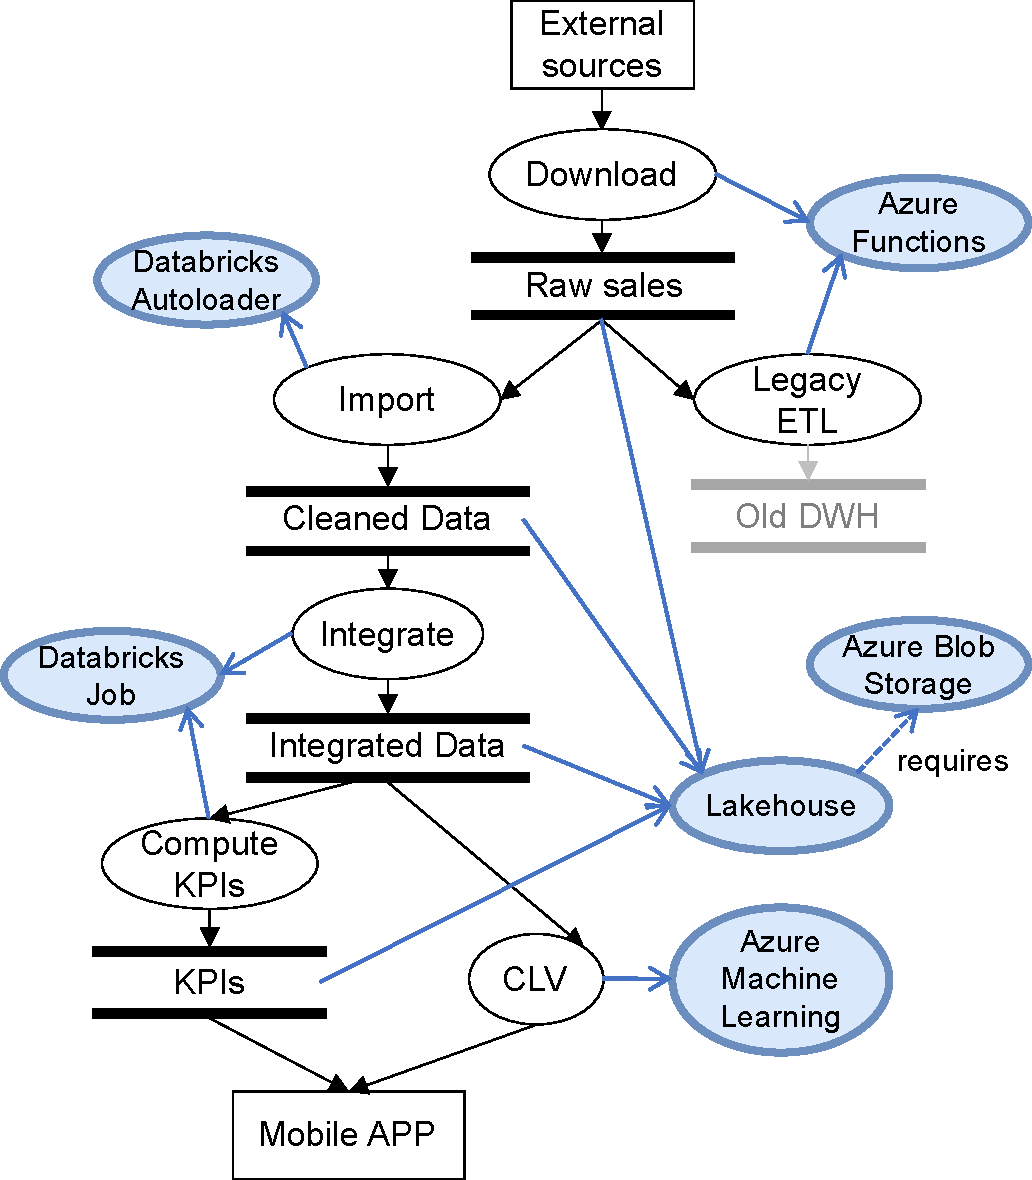
\includegraphics[width=0.55\textwidth]{parts/methods/images/ico.pdf}
    \caption{Matched graph and selected services for case study \#1.}
    \label{fig:pdd-cs1}
\end{figure}

Here follows a description of the Case Studies (CS). Their DFDs along with their blueprints are represented in \Cref{fig:pdd-cs1,fig:pdd-cs2}.

\begin{example}[CS\#1: creating a KPI factory]
Starting from an on-premises data warehouse that has reached a performance plateau, a sales company aims to create a KPI factory: a centralized system where all KPIs are incrementally computed. The data warehouse only supports KPI calculations four times a day, but the company needs more frequent updates. The KPI calculation starts with sales data being drawn from external sources every hour via HTTP API. This data is then stored in its original format, cleaned, integrated, and made usable on a multidimensional engine. It is crucial to store the data at each processing step to facilitate different levels of analysis. For instance, the integrated data is utilized for machine learning models to estimate customer lifetime value. The calculated KPIs are sent to applications managed by client advisors for client-telling actions and are accessible via JDBC connectors. Additionally, the (old) data warehouse must continue to be updated with new data through its legacy ETL procedure. Since the on-premises data warehouse is out of the scope of the platform, we grayed it out in \Cref{fig:pdd-cs1}.
\end{example}

\begin{figure}[htbp]
    \centering
    %[FIGURE: matched graph e servizi selezionati per il caso studio 2 (customer lifetime value forecasting)]
    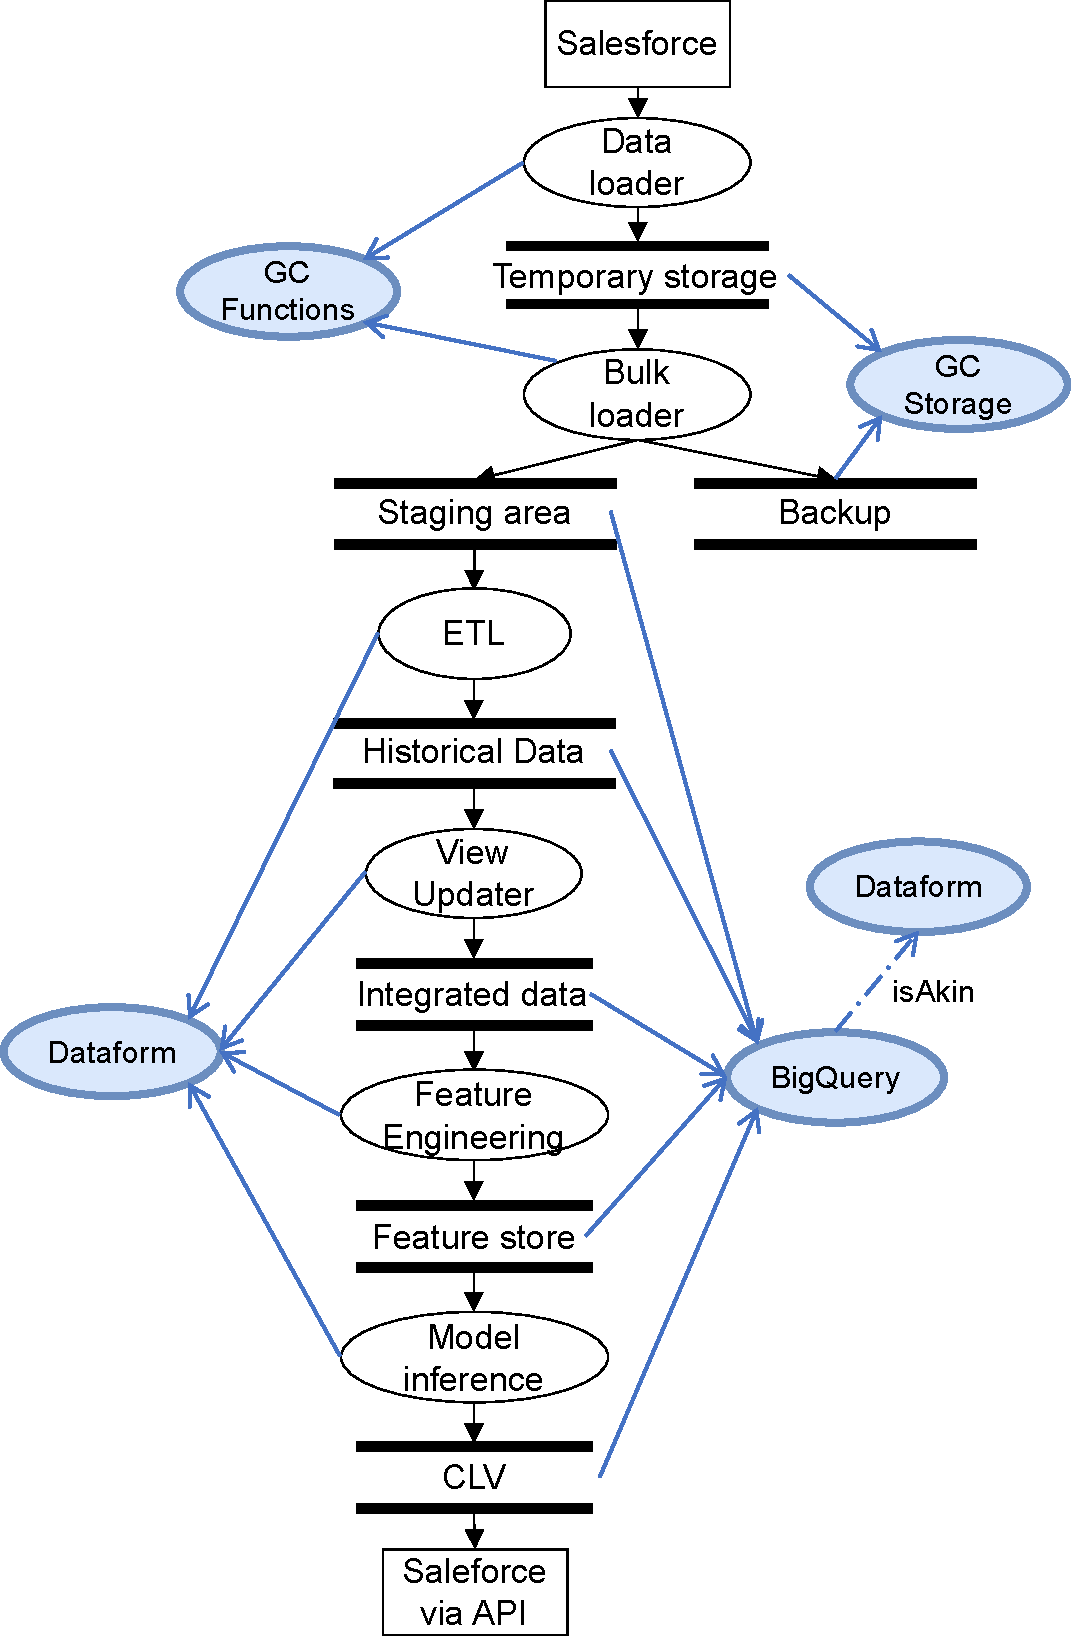
\includegraphics[width=0.5\textwidth]{parts/methods/images/technogym.pdf}
    \caption{Matched graph and selected services for case study \#2.}
    \label{fig:pdd-cs2}
\end{figure}

\begin{example}[CS\#2: forecasting customer lifetime value]
From a Salesforce CRM ecosystem, users' data is extracted every thirty minutes via API calls leveraging a change-data-capture mechanism and is stored in .csv files. Daily, such .csv files are then pushed into two buckets: the first acts as an ingestion backup storage while the other serves as a staging area. From the latter on, data flows through an ETL procedure that updates both the historical trend and the real-time view of each user. The output of the ETL procedure is transformed through feature engineering and fed to a machine learning model predicting the customer lifetime value. Finally, inferred data is filtered and copied into the Salesforce CRM via a custom application.
\end{example}

All in all, we draw the following conclusions.
\begin{itemize}
    \item \textbf{Blueprints effectiveness.} The blueprints returned by our system are compatible and overlap with the ones actually adopted by the companies. In CS\#1, our solution matches the company's solution with 6 services out of 7. The only difference is \serv{Azure Machine Learning}. The company preferred to keep the machine learning activity within the Databricks ecosystem rather than in Azure. This could be fixed by imposing a mandatory service to fulfill the \serv{CLV} process. Similarly, in CS\#2 we matched 4 services out of 5 since we adopted \serv{Google Cloud Functions} for the \dfd{Data Loader} process but the company preferred to use \serv{GSUtils} within the \serv{Google Cloud CLI} (command line interface). \serv{BigQuery} is akin to \serv{Dataform} since \serv{Dataform} operationalizes scalable data transformations pipelines in \serv{BigQuery} using SQL \cite{dataform}.

\item \textbf{Methodology effectiveness.} The requirement analysis was smooth and the staff from the two companies had no problem describing the data-processes and answering questions needed for tagging. The case study from Company1 required a refinement of the DFD since it involved several organizational constraints. For instance, the \dfd{Raw Sales} repository is handled by a different department than the one handling the repositories \dfd{Cleaned Data}, \dfd{Integrated Data}, and \dfd{KPIs}. This organizational constraint impacts the blueprint. On the one hand, if the two departments were willing to share the same technological solution, then all repositories could be implemented by \sf{Lakehouse} even though their management would be separated (as in \Cref{fig:pdd-cs1}). On the other hand, if \dfd{Raw Sales} should be detached from the following part of the pipeline, then it would implemented using \serv{Azure Blob Storage} rather than \serv{Lakehouse} (being a data lake that is not eventually connected to a data warehouse, we correctly discard \serv{Lakehouse} as a possible implementation).
\end{itemize}
Both companies acknowledged that selecting services for a project is highly complex and that staying up to date about service provider offerings requires considerable time and effort. Overall the experts were enthusiastic about the approach and highlighted the following strengths: (i) it can support and train young designers for the creation of blueprints, (ii) it can remove bias in the selection of services (e.g., consultants mainly working with a hyperscaler could tend to prefer services that hyperscaler), and (iii) it is an objective approach to compare different blueprints. Although the blueprints are not perfectly overlapping, experts claim that our blueprints are correct from a technical and technological point of view. However, what could be improved in our approach is the integration of more organizational, political, or even familiarity constraints that could bias the service selection. Our approach partially addresses these issues during the augmentation of the matched graph (e.g., with properties \lbl{IsAkin}, \prop{Mandatory}{True}, and \prop{Preferred}{True}) but could benefit by allowing further expressiveness.

\subsubsection{Efficiency}

We test how our approach scales up to bigger cloud ecosystems and data pipelines, both translating into bigger service and DFD graphs with more nodes and relationships.

To do so, we implement additional synthetic pipelines (i.e., DFDs with increasing nodes $|N^D|$) that share the service ecosystem and the taxonomy of tags. DFDs are created using a tree structure that is randomly expanded until a given number of nodes is reached. The shared service ecosystem contains 200 services with a compatibility rate of 95\% (that is, each service is compatible with 95\% of the others). Each service is enriched with a pair of tags randomly extracted from the shared taxonomy (using a uniform distribution). Finally, each node in the DFD is enriched with a pair of tags selected from the set of tag pairs previously assigned to the services within the service ecosystem. This ensures that every node in the DFD is implemented by at least one service.

To assess the scalability of the approach, the synthetic pipelines differ by a factor of 5x in terms of the number of nodes composing each DFD, starting with DFDs of 10 nodes (as for the real pipelines described in \Cref{sec:pdd-val}) up to 250 nodes.\footnote{We use DFDs of 250 nodes to stress our system although we believe that they are hardly manageable in real applications.} For each number of nodes $N^D \in [10, 50, 250]$ we randomly generate 10 DFD graphs and \Cref{tab:pdd-scalability} and \Cref{fig:pdd-scalability} summarize the average results. Overall, our approach scales well to scenarios involving 200 services and 250 data processes/repositories in the DFD, with a computational time of less than 10 seconds. The time necessary for augmentation and pruning is negligible, whereas matching dominates the total time (93\% for 250 nodes). Matching could be improved by further optimizing GraphDB since the match is automatically solved by the reasoner.

\begin{table}[htbp]
    \centering
    \caption{Breakdown of performance (in seconds) by increasing the nodes of the DFD.}
    \label{tab:pdd-scalability}
    \begin{tabular}{c|ccc|c}
    \toprule
    $|N^D|$ & Match & Augment & Select & Total \\
    \midrule
    10 & 0.22  & $4 \cdot 10^{-5}$ & 0.17 & 0.38 \\
    50 & 0.87  & $4 \cdot 10^{-5}$ & 0.26 & 1.13 \\
    250 & 7.23 & $5 \cdot 10^{-5}$ & 0.53 & 7.76 \\
    \bottomrule
    \end{tabular}
\end{table}

\begin{figure}[htbp]
    \centering
    %[FIGURE: stacked bar chart delle performance (match/augment/select) al crescere della dimensione del DFD]
    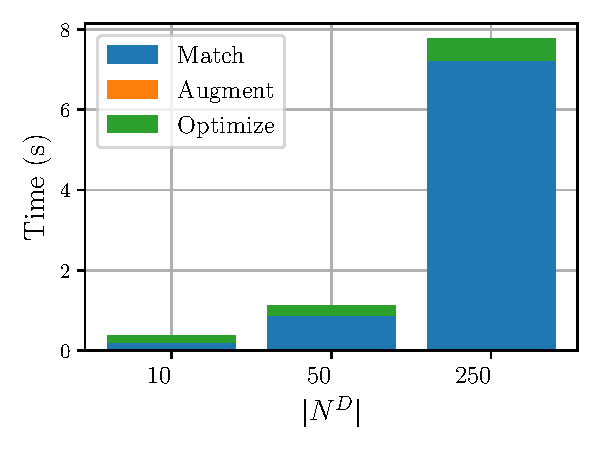
\includegraphics[width=0.7\textwidth]{parts/methods/images/stacked_bar_chart.pdf}
    \caption{Performance by increasing the size of the DFD.}
    \label{fig:pdd-scalability}
\end{figure}

\subsection{Related Work}
\label{sec:pdd-related}

Understanding which ``building blocks'' should be part of a data platform is nontrivial. Several functional architectures (system representations that focus on its functions and their interactions) have been proposed. NIST designed the Big Data Reference Architecture \cite{chang2019nist} which comprised vendor-, technology- and infrastructure-independent logical functional components that are necessary for managing and processing big data (data provider, data consumer, system orchestrator, big data application provider, and big data framework provider). Lambda \cite{DBLP:conf/bigdataconf/KiranMMDB15} is an architecture designed to handle massive quantities of data by taking advantage of both batch and stream-processing methods. Kappa \cite{kreps2014questioning} overcomes some limitations (e.g., ``redundant'' batch and streaming implementations) of Lambda by using a pure streaming approach with a single code base. While these architectures define functional components necessary for (big) data platforms, they are abstract and do not address the problem of selecting the optimal services necessary for designing, implementing, and deploying working data platforms.

Cloud service providers such as Amazon \cite{aws}, Google \cite{gcp}, and Microsoft \cite{azure} provide ecosystems of independent and interoperable services. While ecosystems enable easy deployment of data pipelines, choosing the \textit{optimal} services is hard: (i) each provider offers different services, (ii) a shared categorization and organization of services is missing, and (iii) it is hard for the users to understand which services are needed based on their data-driven processes \cite{DBLP:journals/jnca/SunDHHC14}. Some multi-objective optimization techniques have been proposed, where users express requirements and preferences (e.g., minimal QoS) about single services \cite{DBLP:conf/ncca/CavalcanteLBCDP11,DBLP:journals/cluster/NejatMVB22,DBLP:journals/jss/LuY18}, cloud deployment models (public and private) \cite{DBLP:journals/tcc/Garg22}, and service providers \cite{DBLP:journals/eswa/KarKPK23,DBLP:journals/cluster/TomarKG23}. Finally, domain languages and ontologies have been introduced (e.g., \cite{DBLP:conf/webi/NouraG19}) to enable some service composition (e.g., \cite{DBLP:journals/jsan/MahfoudhCS21}).

With respect to these works, the novelties of our approach are (i) the introduction of a methodology to enable data platform design, (ii) a computer-aided approach to support designers in their choices, and (iii) process-driven optimization to select the optimal blueprint out of many data flows, even from multiple stakeholders.

\subsection{Conclusion and Future Directions}
\label{sec:pdd-conclusion}

The design of data platforms is a nontrivial task. {\color{red}This chapter} introduced a methodology to aid designers in selecting the optimal services (out of a service ecosystem) supporting data-driven processes from multiple stakeholders (e.g., partners in a research project), and addressed such selection as a facility location optimization problem. Our approach can match and select single services as well as design patterns (e.g., Lakehouse to replace both data lakes and warehouses), it supports additional constraints (e.g., mandatory and affinity), and the produced blueprints have been successfully compared with the ones recommended by expert designers.

We believe that the expressiveness of the approach can still be improved as follows. \textit{Expressiveness}: introduce more advanced constraints to support organizational and political factors in the design of the blueprints. \textit{Resource provisioning}: additionally to selecting the services, a complete approach should also consider how many instances of a service are required (to do so, a cost model should be studied). \textit{Metadata integration}: while catalog and meta-data management services do not directly introduce functionalities for data transformation and exploitation, the design should also recommend services helping in the management of the platform itself \cite{francia2021moses}.

{\color{red}
The metadata-integration direction identified above is taken up directly in the following chapter, which investigates how Large Language Models can support users in querying the metadata of a data-intensive system -- in that case, a data warehouse -- without requiring expertise in its underlying schema, continuing this thesis's preliminary exploration of the mechanisms required for Digital Twins to be understood, and eventually integrated, beyond the boundaries of a single deployment.
}

\section{LLM guided metadata exploration}
\label{sec:llm-guided-metadata-exploration}\
\input{parts/methods/chapters/llm4bi.tex}